%第3-2章
\section{要求定義}
続いて、本システムがどのような機能を持ち、利用者にどのように利用されることを想定するかを、図\ref{usecase}のユースケース図を用いて説明する。

\begin{figure}[H]
	\centering
	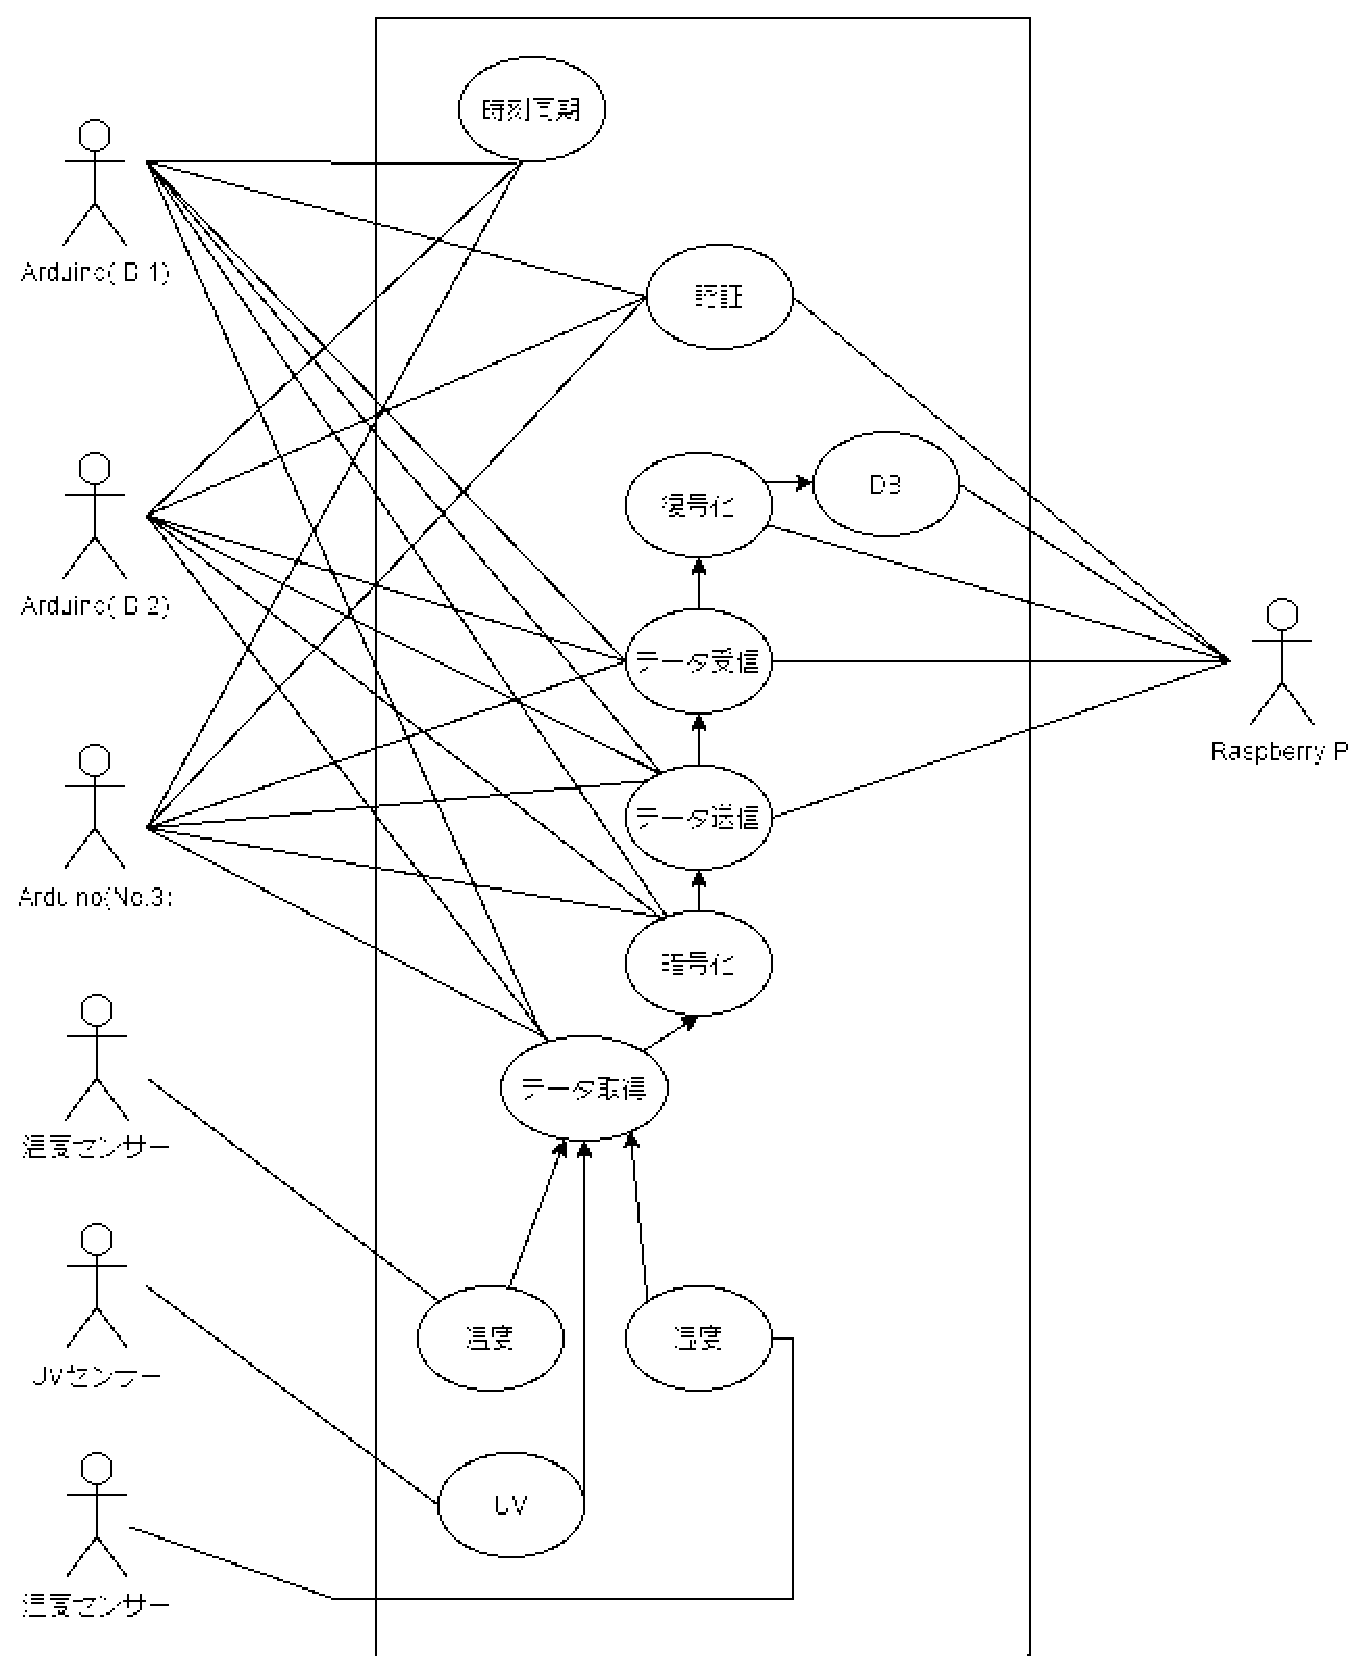
\includegraphics[width=10cm]{usecase.eps}
	\caption{ユースケース図}
	\label{usecase}
\end{figure}

図\ref{usecase}のユースケース図では、「室内環境を監視する」「部屋情報を登録する」「入室危険度の確認」「換気要請の受け取り」「室内環境状態の表示」という5つのユースケースを挙げている。3.1章でも述べたように、本システムは、デバイス類の電源等の準備が完了すれば自動的に稼働する。そのため、利用者側で事前に準備することは部屋情報をシステムに記録しておくということのみである。部屋情報とは、部屋の広さと何平方メートルに1人が滞在可能とするかという運用ルールの2つのデータのみであり、具体的には数値データである。この数値は、一般の利用者が勝手に書き換えてよいものではないが、今回はマイコンボードを用いていることから、管理者がマイコン内の所定のファイルにこれら2つの数値を記録しておき、システムが読み出すという仕様になっている。

システム稼働後にも、基本的には一般利用者がシステム利用のために、システム側に働きかける必要はなく、感染予防のサポートのため、システム側からの利用者に対する能動的な働きかけを中心とする。ユースケース図では、いずれのユースケースもユーザ側のアクションとして、能動的な表現を用いているが、ユーザの働きかけに関わらず、決められたスケジュールで機能する。こういった仕様となったのは、本システムが能動的に利用者に対して情報提供を行うことを重要視したためである。また、本システムは1つの部屋という単位で、同時に多くの人を対象として機能しなくてはならないという点からも、各自で確認しなければならないような情報共有の方法よりも、リアルタイムに必要な情報だけを、システム側からの働きかけで提供することを優先している。

ここで提供する情報は、室内の感染リスク状況・入室の危険度、換気要請、室内環境状態の3つがあるが、どのような情報をどのような基準に沿って提供すればよいかという点に関しては、要求定義の段階で繰り返し議論された。この点が多くの議論を要した要因は、室内環境というものが、部屋に滞在する人数や換気状況などによって目まぐるしく変化するものであり、何よりも感染予防のためには、情報提供のスピード感というものが損なわれてはならず、利用者側がとるべきアクションが明確にならなければ、真に価値ある情報を提供することにはならないためである。

初期段階では、室内に滞在する人の数にはそれほど着目しておらず、二酸化炭素濃度の高さに応じて部屋の感染リスクを段階的に定義し、利用者には警戒レベルとして数値を示すというものであったが、二酸化炭素濃度のみに着目した環境評価であれば、既存のシステムが多く存在しているはずであるし、警戒レベルの定義に関しても、システム内部で定められているのみならば、受け取った側が感染の危険度を実感しづらいはずである。以上のように情報提供に関しては、その質と迅速性を特に重要視した。

ここで、リアルタイム性の高さと、精度の高さを併せ持つ、人数推定のために用いた物体検出手法「Yolo」について簡単に説明する。物体検出手法Yoloとは、それまで一般的には異なるモデルの組み合わせで行われていた、画像の領域推定と分類の処理を1つのCNNで完結し、リアルタイム処理を可能とする高速な物体検出手法である。実際にYoloでは静止画だけでなく、動画に対しても物体検出を適用可能であり、非常に高速な処理を可能としている。本システムでは、すでに説明したように、3分おきのデータ取得とその分析による情報提供を行う。そのため、高速な画像処理を行うためにエッジサーバ側にJetson nanoを選定しており、画像処理によって部屋全体の滞在人数を高速に数えることを目標として設定した。なお、自身はこの技術を感染予防サポートシステムにおける情報取得の1つの手法として、システムから利用できるよう、人数推定機能担当者の担当部分をシステムに統合するなどしたものの、その中身に関しての詳しい説明はここでは省略する。

このように私たちは、提供された情報によって利用者が的確な感染予防対策を講じるために求められる情報とは何か、またその情報がどのような尺度で導き出されるべきであるかの議論を、特に重点的に行った。ここから、最終的に定まった情報提供の指針について述べる。

まず、利用者に提供する情報の導き出し方としては、大きく分けて以下の2点が基本方針として定められた。

\begin{itemize}
	\item 二酸化炭素濃度値の高さに応じて部屋の警戒レベルを導出する。
	\item 警戒レベルの高さに応じて、部屋に滞在できる人数を制限し、室内の滞在人数が、この警戒レベルごとの制限人数に適しているかを評価する。
\end{itemize}

先ほども述べたように、二酸化炭素濃度値のみを監視の対象としたシステムでは、情報の受け取り手がその情報のみをもとにして取れるアクションは、基本的に換気のみとなる。しかしながら、このようなシステムはすでに多く存在していることが確認でき、3つの密のうち、密閉の対策にしかならず、本システムで実現しようとする3密回避のための機能を満足できない。密集と密接に対しアプローチするために欠かせない情報は、部屋に滞在する人数の情報であるため、二酸化炭素濃度と室内の滞在人数とを併せて導き出される情報を提供する必要がある。したがって、室内の滞在人数に関しても、部屋の広さと運用のルールから求められる、その部屋に滞在可能な規定人数と、警戒レベルごとに制限される滞在可能人数を基準とした評価を行うこととした。

以上のような考えから、最終的に利用者に提供する基本的な情報を、二酸化炭素濃度値と室内の滞在人数というデータに基づいた分析結果として、赤黄緑の3色の信号によるリスクのレベルの通知と、二酸化炭素濃度上昇時の、ブザーを用いた換気要請に絞った。ただし、新型コロナウイルスと湿度の関連についても、様々な観点から多くの研究がなされており、理研などでの研究によって、湿度が低いほど飛沫の拡散が大きくなるとの成果が求められている点に着目し、本システムでは部屋の湿度が30\%を切った場合に発出する警告を、付加的な情報として提供することとなった。

私たちはこれら2 つの情報が、3 密回避の基準となり得る、意味ある情報となるはずであると考えた。まず、二酸化炭素濃度の高さに関わらず、部屋に滞在可能な規定人数を越えた人数が部屋に滞在している場合には、3 色のリスクの信号は最も危険な状態を示す赤になり、密集、密接を避けるために、滞在・入室が可能な人数を制限できる。また、二酸化炭素濃度の上昇を受けて警戒レベルが高まっている場合には、部屋に滞在可能な人数がより少なく設定されることから、人数に変動がなくてもリスクの信号が変わる場合がある。反対に二酸化炭素濃度に大きな変動がなくても、室内に滞在する人数が増えたことで、滞在可能な人数上限を越え、リスクの信号が変わる場合も考えられる。これら2 つのケースでは、利用者に、換気によって二酸化炭素濃度を下げ、警戒レベルを緩めるか、滞在する人数を減らすという選択をとることを意識づけることができる。室外からも入室の際の目安となる情報を得られ、感染リスクの更なる高まりを防ぐことが可能となる。何よりも、この情報提供の方法が、最もシンプルでわかりやすいという点からも、有効な感染予防サポートシステムとして機能すると考えた。

以上を踏まえ、本システムにおける情報収集と情報提供の2点について、簡単にイメージを図\ref{analysisimage}に示す。

\begin{figure}[H]
	\centering
	\includegraphics[width=15cm]{analysisimage.eps}
	\caption{情報収集・分析イメージ}
	\label{analysisimage}
\end{figure}

図\ref{analysisimage}では、部屋の感染リスクを示す警戒レベルと、部屋の警戒レベルを決定づける二酸化炭素濃度値の基準、警戒レベルごとに制限される滞在可能人数の3項目の関連を表している。本システムでは、室内の複数箇所で観測した二酸化炭素濃度値のうち、最も換気状態が悪いと考えられる地点の値を代表値とし、その値に応じて部屋の警戒レベルを5段階で評価する。ここでは、部屋の警戒レベルを最高レベルとする場合の二酸化炭素濃度を、厚労省が建築物衛生法などで定める基準値1000ppmとして、各警戒レベルと二酸化炭素濃度基準値を段階的に設定した。二酸化炭素濃度値が上がるにつれて換気状態は良好でないと判断されることから、警戒レベルを上げるとともに、室内に滞在できる人数も段階的に制限する。二酸化炭素濃度が700ppm未満の場合は、標準警戒レベルとし、部屋の広さと部屋の運用ルールから求められる部屋の滞在可能規定人数からその95\%未満までの人数を、滞在可能人数の目安と定める。同じように、これよりも高い警戒レベルでも、滞在可能人数の上限と下限が定められる。ただし滞在可能人数の下限とは、ここで定める安全水準を満たすことのできる人数の、範囲の下限を意味する。

システム内ではこのような分析がなされているものの、警戒レベルや現在の二酸化炭素濃度などの情報はシステム内部で導き出されているに過ぎない。先ほども述べたように、実際に提供されるのは換気要請と室内の感染リスクの情報であり、二酸化炭素濃度の上昇によって室内の警戒レベルが上昇した際の換気要請と、室内に実際に滞在している人数が、現在の警戒レベルによって定められている滞在可能人数に適合しているかどうかによって、3色LEDによるリスクのレベルの通知がなされる。具体的には、その時点の部屋の警戒レベルで定められている、滞在可能下限人数より少ない人数が滞在している場合には緑、下限人数以上上限人数未満が滞在している場合には黄、上限人数以上が滞在している場合には赤のLEDが点灯し、部屋の感染リスクを通知する。またこの室内感染リスクは、室外から見ることができる部屋への入室危険度と対応しており、部屋の感染リスクが高まっている場合の入室を制限することができる。利用者はこれらの情報をもとに、換気を行うか滞在する人数を調整するといった対応をとらなくてはならない。

続いて、よりアクターとシステム間の対話の様子を明確に示すために、アクター側の振る舞いを文章で記述したユースケース記述を図\ref{usecasekijutu}に示す。

\begin{figure}[H]
	\centering
	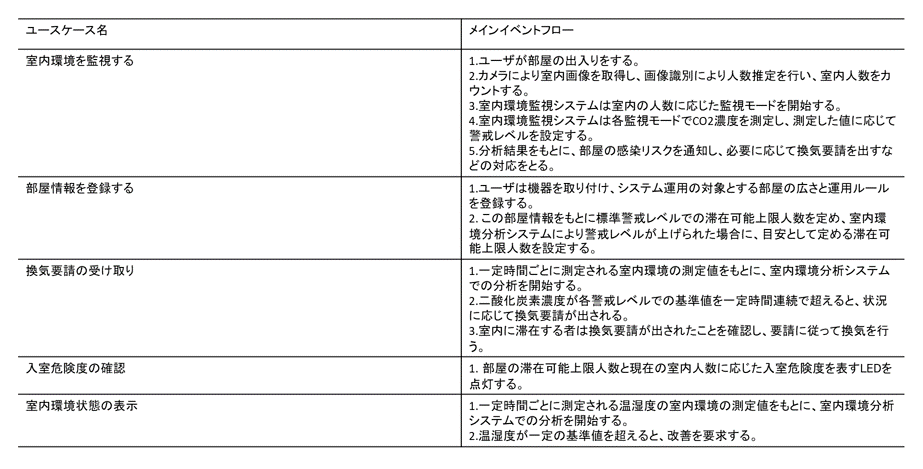
\includegraphics[width=15cm]{usecasekijutu.eps}
	\caption{ユースケース記述}
	\label{usecasekijutu}
\end{figure}


図\ref{usecasekijutu}のユースケース記述からもわかるように、システムの利用者は部屋の出入りなどで、室内環境に変化を与える働きを持つが、多くの機能はシステム側が能動的に提供するものである。

以上の内容から、ユースケース図、ユースケース記述に挙げた5つのユースケースのうち、特に一般利用者に関わりのある4つのシナリオをもとに、総合テスト項目として表\ref{sougoutest_koumoku}の項目を挙げた。

\begin{table}[H]
	\centering
	\caption{総合テスト項目}
	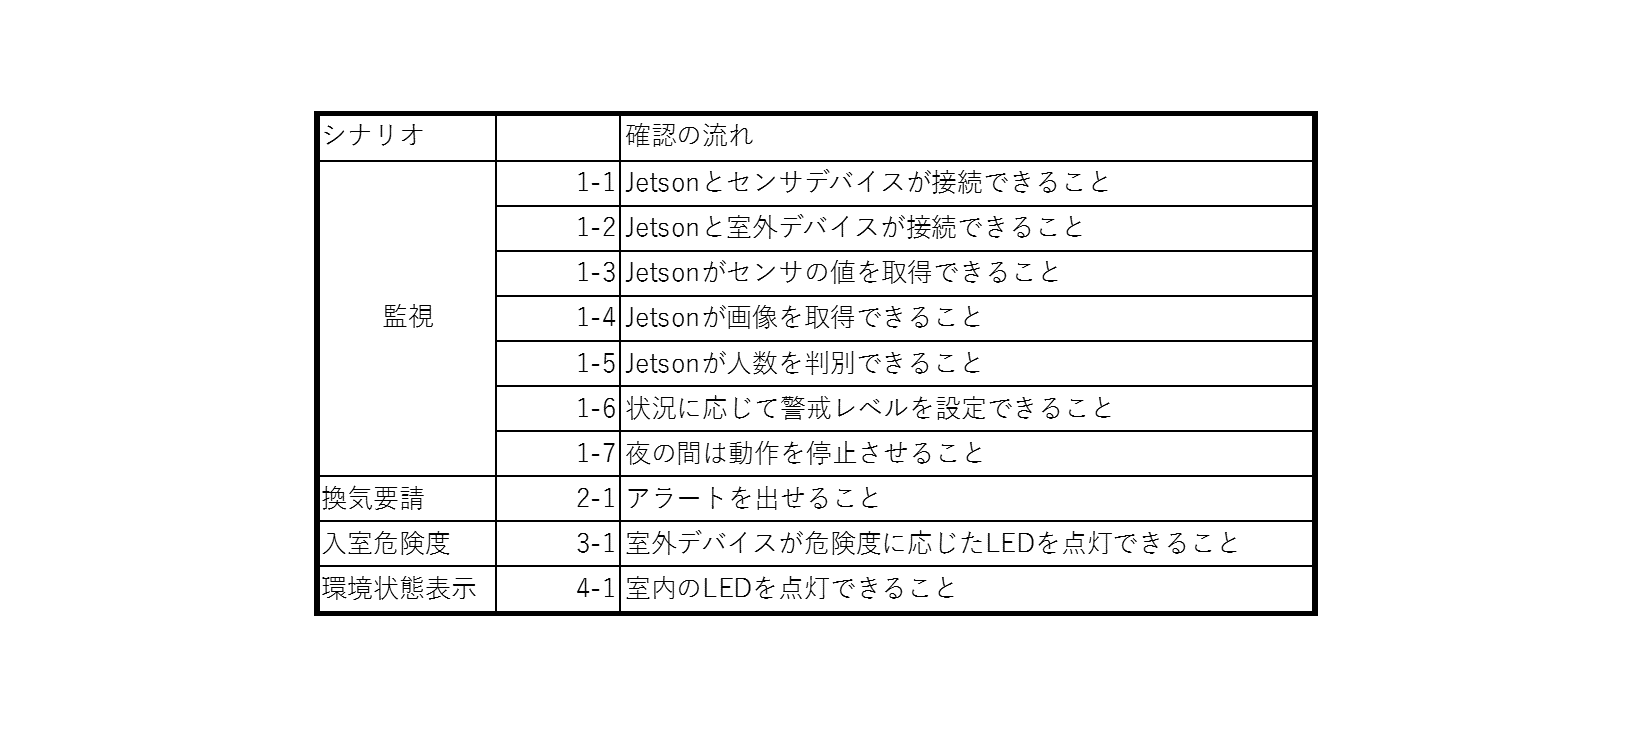
\includegraphics[width=15cm]{sougoutest_koumoku.eps}
	\label{sougoutest_koumoku}
\end{table}

